\chapter{Methodology}
To ensure the success of this project a basic plan of action was created. The following diagram shows the critical phases of the project.

\begin{figure}[!ht] 
\captionsetup{width=0.8\linewidth, font=small}  
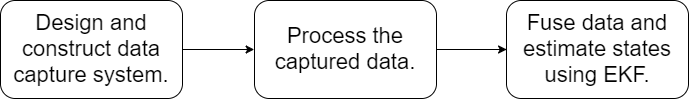
\includegraphics[width=0.8\linewidth]{figures/planOfAction.png}
  \caption{Diagram showing the progression and dependence of the major stages of this project}
\label{fig:planOfAction}
\end{figure}


Due to the availability of equipment, financial limitations and time  

  
\section{System Design}
This section is dedicated to defining and understanding the specifications of the data capture system. The system will consist of 4 cameras and an IMU mounted to the torso of the subject. the cameras will record the legs of the subject while the IMU will log inertial data from the body of the subject.

Due to the availability of equipment provided by the Mechatronics Lab the following equipment was chosen as the main components to use in the system:


\begin{table}[!ht]
\label{equipment-table}
\begin{tabular}{llll}
Item		& Selected Equipment		   & From		  \\
Camera      & 4 GoPro Hero Session Cameras & \cite{gopro} \\
IMU         & 1 Sony Xperia Z3 Compact     & \cite{sony}  \\
Chest Mount & 1 Action Mount Chest Mount   & \cite{actionmounts}   
\end{tabular}
\caption{The main components used}
\end{table}

The specifications of this data capture system has been defined as:
\begin{itemize}
\item Stereo housing to hold the cameras.
\item Chest mount to hold the cameras and IMU.
\item 
\item 
\end{itemize}

\section{Modelling the Lower Limbs}
talk about the model here

\section{Experimental Details}
The data was captured during a short

\section{Sensor Fusion}
asdfasdkfjasldfk

\section{Limitations}
system shortcomings
experimental shortcoming
model shortcomings







 



















